\section{Underlying Work}
\label{sec:underlying}

In this section we discuss the underlying work by \ca{sanchez2019can}. We talk about the methodology they use and the
results they achieve with their strategy.

The main focus of the underlying work is not to evaluate whether websites comply with the law, but rather to evaluate
the impact of the GDPR on the ability of a user to control their privacy online.

\subsection{Methodology}
\label{subsec:methodology}

The target list of their analysis are the Alexa top-1M websites, a list by amazon showing the top 1 million websites with
the most traffic according to the Alexa Traffic Rank. From this list, they look at 2000 websites across different
categories from some of the top traffic websites. The location of the website is determined by the top-level domain 
if it corresponds to a country and otherwise through IP geolocation with \texttt{ip-api.com} despite being inaccurate at
times \cite{weinberg2018catch}. They chose the top 100 websites of a category with the top 20 categories being determined
by Symantec RuleSpace~\cite{symantec} resulting in 2000 websites. \autoref{tab:websites} shows the categories broken
down by region. We can observe that most of the websites reside in the USA. In the remainder of the evaluation we will omit the
results comparing the different categories since this would be outside the scope of this report.

\begin{table}
    \begin{tabular}{ l  r  r  r  r}
        \hline
        & EU & USA & China & Others\\
        \hline
        Business & 18\% & 52\% & 8\% & 21\%\\
        Entertainment & 24\% & 53\% & 5\% & 18\%\\
        Finance & 30\% & 27\% & 10\% & 33\%\\
        Food & 27\% & 49\% & 10\% & 14\%\\
        Gaming & 28\% & 53\% & 8\% & 11\%\\
        Government & 28\% & 32\% & - & 40\%\\
        Health & 18\% & 57\% & 16\% & 9\%\\
        Hobby & 21\% & 56\% & 7\% & 16\%\\
        Kids & 35\% & 57\% & 1\% & 7\%\\
        News & 25\% & 35\% & 11\% & 29\%\\
        Politics & 15\% & 65\% & - & 20\%\\
        Pornography & 31\% & 52\% & 1\% & 16\%\\
        Real Estate & 26\% & 37\% & 12\% & 25\%\\
        Religion & 12\% & 63\% & - & 25\%\\
        Science & 35\% & 47\% & 7\% & 11\%\\
        Shopping & 35\% & 30\% & 10\% & 25\%\\
        Sports & 48\% & 25\% & 1\% & 26\%\\
        Technology & 11\% & 66\% & 9\% & 14\%\\
        Travel & 37\% & 36\% & 9\% & 18\%\\
        Weapons & 15\% & 72\% & 1\% & 12\%\\
        \hline
    \end{tabular}
    \caption{Websites by region and category. Table by \citeauthor{sanchez2019can}~\cite[Tab.~1]{sanchez2019can}}
    \label{tab:websites}
\end{table}

The data collection was done manually. This means that \citeauthor{sanchez2019can} went through all the 2000 websites
manually with a browser and noted features of the website. The only thing that was automated was the collection of the
cookies while visiting the website via a browser extension. By doing this manually, you are less likely to miss any cookie notice.
Cookie consent notices can differ tremendously from one website to another making it hard to
automate this task. On the other hand, collecting the data manually makes it harder to recreate the data they produced
and harder to look at different features afterwards because it takes a long time to do this task manually.
Manual analysis provides better error resistance but is
less flexible and practical than automated analysis. The data they collect are the cookies set before interacting with the
consent notice, the type of consent notice, the privacy policy and the cookies set after rejecting trackers if possible.
The different types of consent notices are:
\begin{enumerate}[a)]
    \item \emph{Anyway}: Users are just informed that they are being tracked.
    \item \emph{AutoAccept}: Users are informed that by continuing to browse they accept tracking.
    \item \emph{OnlyAccept}: There is only an accept button.
    \item \emph{AcceptReject}: There is an accept and a reject button.
    \item \emph{JustSettings}: There is a more complex settings dialog.
\end{enumerate}
Cookie consent notices can be blocking and non-blocking meaning that you can access the website while the consent notice pops up for
non-blocking, and you cannot access the website until you have made a choice for blocking cookie consent notices. For
websites which link to third-party opt-out services(e.g. youronlinechoices), they used the service and observed the
cookie behavior.

The identification of tracking cookies was done through measuring the entropy of the value of a cookie with
\texttt{zxcvbn}~\cite{wheeler2016zxcvbn}, a tool for password strength estimation.
If the entropy is high enough to distinguish you from 1 Billion people, they
consider it a tracking cookie. This is a rather new approach to the problem of identifying tracking cookies.
On one hand you can detect cookies which with other methods could have been missed, but on the other hand you can get false positives
where the cookie was not a tracker, but it was still classified as one. The latter is not a problem in our case since the
GDPR specifies that cookies which carry information that in theory could identify you still require consent except if
they are essential (e.g. shopping cart) even if they are not used as tracking cookies. In the evaluation
\citeauthor{sanchez2019can} do not use any functionality of a
website which requires any essential trackers (e.g. like shopping carts) meaning that there is almost no possibility
that they should get an essential tracking cookie.
A more common approach is to make use of lists of known third-party trackers. This approach cannot reliably identify
first-party trackers and can miss some unknown third-parties. \citeauthor{sanchez2019can} use third-party tracker lists
to classify their found trackers (first-party, third-party and unknown).

The GDPR requires privacy policies to be readable. A privacy policy is a legal document that discloses how
a website handles the data of a user accessing the site. Privacy policies are typically found on the bottom
of a website through a link. Often, the privacy settings (e.g. cookie control) are only presented
in the privacy policy section of a website. While performing their manual analysis on consent notices,
\citeauthor{sanchez2019can} also copy the privacy policy of a website if present. They evaluate the reading difficulty of
privacy policies with
two metrics, the \emph{Flesch Reading Ease Score} (FRES)~\cite{flesch1948new} and the \emph{Flesch-Kincaid Reading
Level} (FKRL)~\cite{kincaid1975derivation}. Both metrics evaluate the difficulty of texts through number of syllables
per word and sentence length. A FRES of about 50 could be seen as an average reading difficulty. The FRES has an upper
bound of 121.22 (greater equals easier text) and no theoretical lower bound. The FKRL can be interpreted as the years of
formal education you need to fully understand a text. The FKRL has a lower bound of -1.3 and no
theoretical upper bound. \ca{jensen2004privacy} also use these metrics making it easy to compare their results to the
results of this paper.

\subsection{Evaluation}
\label{subsec:eval}

In this subsection we highlight some of the main results of the underlying work.

\subsubsection{Tracking}

\begin{figure}
    \centering
    \begin{subfigure}[b]{.5\textwidth}
        \centering
        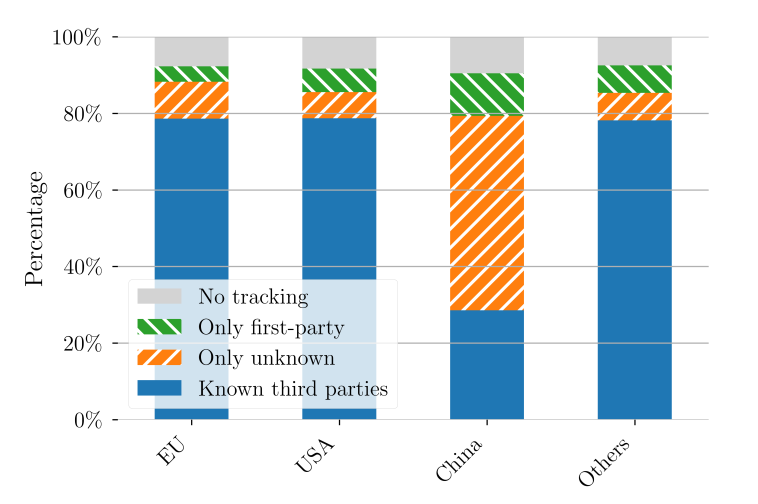
\includegraphics[width=\textwidth, scale=0.27]{figures/tracking_kind_trans.png}
        \caption{Kind of tracking observed.\\Figure by \citeauthor{sanchez2019can}~\cite[Fig.~1]{sanchez2019can}.}
        \label{fig:tracking_kind}
    \end{subfigure}
    \begin{subfigure}[b]{.5\textwidth}
        \centering
        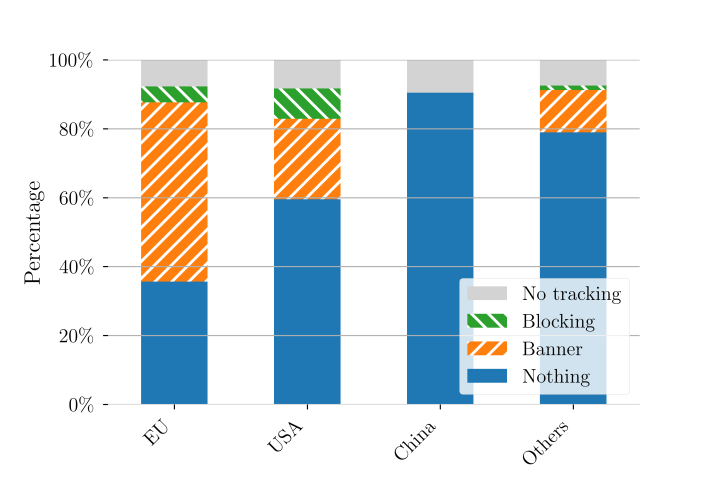
\includegraphics[width=\textwidth, scale=0.3]{figures/cookie_notice_size_trans.png}
        \caption{The size of the cookie notice.\\Figure by \citeauthor{sanchez2019can}~\cite[Fig.~2a]{sanchez2019can}.}
        \label{fig:notice_size}
    \end{subfigure}
    \begin{subfigure}[b]{.5\textwidth}
        \centering
        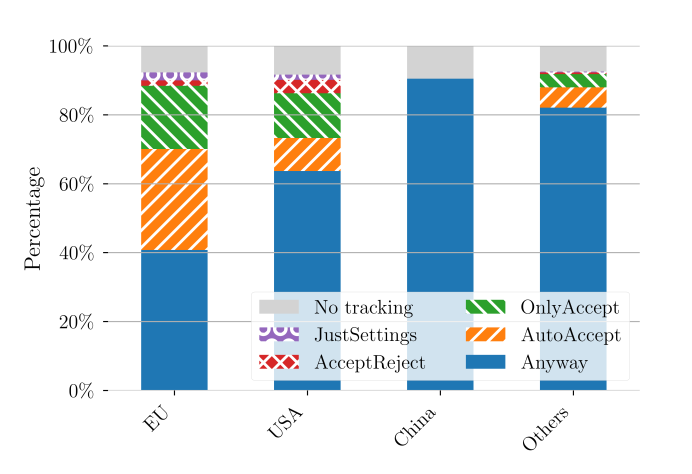
\includegraphics[width=\textwidth, scale=0.3]{figures/cookie_notice_type_trans.png}
        \caption{Type of cookie notice.\\Figure by \citeauthor{sanchez2019can}~\cite[Fig.~2b]{sanchez2019can}.}
        \label{fig:notice_type}
    \end{subfigure}
    \caption{Statistics about cookie tracking and consent notices}
    \label{fig:cookie_stats}
\end{figure}

\begin{figure}
    \centering
    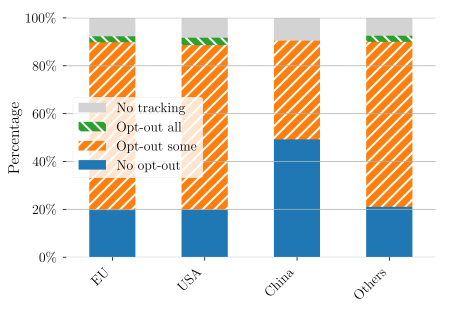
\includegraphics[width=0.48\textwidth, scale=0.1]{figures/third_party_trans.png}
    \caption{Number of cookie identifiers after opt-out through third-party service. Figure by
    \citeauthor{sanchez2019can}~\cite[Fig.~2b]{sanchez2019can}.}
    \label{fig:third_party}
\end{figure}

\autoref{fig:cookie_stats} shows the evaluations of the underlying work that we want to focus on.

\autoref{fig:tracking_kind} illustrates the kind of tracking on the visited websites. We can observe that about 92\% of
the websites perform some kind of tracking. This tracking is done before any consent is given and even after rejecting
tracking cookies (opt-out). Many websites make use of third-party tracking and only a few use first-party tracking. We
can also criticize this figure because we cannot see how many websites that use known third-party tracking also use
first-party tracking because all websites that use third-party tracking are thrown into one category.

\autoref{fig:notice_size} shows the size of the cookie notice differentiating between cookie consent notices which block
you from accessing a website until you have made a choice on cookies, banners which do not block you from browsing the
website and no cookie consent notice (splitting websites that do perform tracking and websites that do not and have no
cookie consent notice). The GDPR specifies that consent must be explicit before any kind of tracking is performed
(opt-in instead of opt-out) meaning that no cookie consent notice despite tracking is illegal.
We can see in \autoref{fig:notice_size} that around 57\% of EU websites and 32\% of US
websites have some form of cookie notice. Chinese websites do not display any cookie consent notice.

\autoref{fig:notice_type} shows the type of cookie consent notice as discussed in \autoref{subsec:methodology}.
We can observe that most websites do not have an easy way to opt-out. The best practices like \emph{AcceptReject} and
\emph{JustSettings} notices are substantially low. If a website has a cookie consent notice, it
most likely just informs the user that cookies are being used. This shows that the GDPR had the impact of getting more
cookie consent notices onto websites, but these are often useless as they are not conform with the GDPR and users are
tracked even if they reject.

\autoref{fig:third_party} depicts the amount of cookies after opting out through third-party servises (e.g.
youronlinechoices). By opting out through third-party services, the number of identifier cookies often decreases
(\emph{Opt-out some}) but only on about 3\% of websites the tracking is completely blocked (\emph{Opt-out all}). We can
however see that third-party opt-out services help in reducing the number of identifier cookies in China. This is an
interesting observation since websites in China typically do not show any cookie consent notice or give a user the
option to opt-out.

\subsubsection{Privacy Policies}
\label{subsub:priv}

\begin{table}
    \begin{tabular}{ l r r r r }
        \hline
        Region & Policies & FRES & FKRL & Length(words) \\
        \hline
        EU & 190 & 57.1 & 10.5 & 2,261 \\
        USA & 617 & 54.5 & 11.2 & 2,698 \\
        All & 849 & 54.1 & 11.1 & 2,250 \\
        \hline
    \end{tabular}
    \caption{Average readability scores of privacy policies. High FRES and low FKRL equals easier texts. Table by
    \citeauthor{sanchez2019can}~\cite[Tab.~5]{sanchez2019can}.}
    \label{tab:policies}
\end{table}

In total, they looked at 849 privacy policies written in English. Other languages are omitted.
\autoref{tab:policies} shows the evaluation they performed on privacy policies. With an average FRES of 54.1, the
policies are still below the threshold of about 60 to 70 which is the score you want for the general public. On the
other hand \ca{jensen2004privacy} provide an average of 34.2 on their dataset in 2004 which shows that privacy policies
have gotten more readable from 2004 to 2019 after the GDPR. We can make the same observation with the FKRL. \citeauthor{sanchez2019can} get to an average
of 11.1 on their dataset and in comparison to the 14.2 by \ca{jensen2004privacy}. Again, the FKRL does not meet the
ideal threshold of about 8, but it still improved over the years. These observations show that the GDPR did not only have
an impact on cookie consent notices, but also on privacy policies. Still the privacy policies of most websites are
rather lengthy (on average 2,250 words). People often do not read the privacy policy due to the length and the
reading difficulty still being too high. \ca{mcdonald2009comparative} have shown in a study that many people still have
problems understanding privacy policies with a FRES of 46.

